\documentclass[aspectratio=169,xcolor=table]{beamer}
\usepackage[utf8]{inputenc}
\usepackage[T1,T5]{fontenc}
\usepackage{amsmath,amssymb,booktabs,array,graphicx,tikz}
\usetikzlibrary{positioning,arrows.meta}

\definecolor{Primary}{HTML}{111B88}
\definecolor{Secondary}{HTML}{101659}
\definecolor{Accent}{HTML}{F2A900}
\definecolor{SoftBlue}{HTML}{EAF2F8}
\definecolor{TextGray}{HTML}{4D5966}
\definecolor{RiskRed}{HTML}{A23B3B}
\definecolor{GoodGreen}{HTML}{26734D}
\mode<presentation>{\usetheme{Madrid}\usecolortheme{default}\setbeamertemplate{navigation symbols}{}}
\setbeamercolor{structure}{fg=Primary}
\setbeamercolor{frametitle}{fg=white,bg=Primary}
\setbeamercolor{title}{fg=white,bg=Primary}
\setbeamercolor{block body}{fg=black,bg=SoftBlue}
\setbeamercolor{block body alerted}{fg=black,bg=Accent!12}
\setbeamercolor{section in head/foot}{fg=white,bg=Primary}
\setbeamercolor{author in head/foot}{fg=white,bg=Secondary}
\setbeamercolor{date in head/foot}{fg=white,bg=Primary}
\setbeamerfont{section in head/foot}{size=\tiny,series=\bfseries}
\setbeamerfont{author in head/foot}{size=\scriptsize}
\setbeamerfont{date in head/foot}{size=\scriptsize,series=\bfseries}
\setbeamerfont{frametitle}{series=\bfseries}
\setbeamerfont{title}{series=\bfseries}
\newcommand{\decklabel}{Contextual ASR -- Scorer}
\setbeamertemplate{itemize item}{\color{Secondary}$\blacktriangleright$}
\setbeamertemplate{itemize subitem}{\color{Accent}$\bullet$}
\setbeamertemplate{headline}{\leavevmode\begin{beamercolorbox}[wd=\paperwidth,ht=2.7ex,dp=1.1ex,leftskip=.35cm,rightskip=.35cm]{section in head/foot}\insertsectionnavigationhorizontal{\dimexpr\paperwidth-.70cm\relax}{}{}\end{beamercolorbox}}
\setbeamertemplate{footline}{\leavevmode\hbox{\begin{beamercolorbox}[wd=.55\paperwidth,ht=2.6ex,dp=1ex,leftskip=.35cm,rightskip=.20cm]{section in head/foot}\usebeamerfont{section in head/foot}\insertsectionhead\end{beamercolorbox}\begin{beamercolorbox}[wd=.27\paperwidth,ht=2.6ex,dp=1ex,center]{author in head/foot}\usebeamerfont{author in head/foot}\decklabel\end{beamercolorbox}\begin{beamercolorbox}[wd=.18\paperwidth,ht=2.6ex,dp=1ex,rightskip=.35cm plus1fil]{date in head/foot}\usebeamerfont{date in head/foot}\hfill\insertframenumber\,/\,\inserttotalframenumber\end{beamercolorbox}}}
\newcolumntype{L}[1]{>{\raggedright\arraybackslash}p{#1}}
\newcommand{\hi}[1]{\textcolor{Primary}{\textbf{#1}}}
\newcommand{\bad}[1]{\textcolor{RiskRed}{\textbf{#1}}}
\newcommand{\good}[1]{\textcolor{GoodGreen}{\textbf{#1}}}
\newcommand{\src}[1]{{\tiny\color{TextGray}[#1]}}
\newcommand{\ra}{$\rightarrow$}
\newcommand{\nbox}[2][block body]{\begin{beamercolorbox}[sep=0.45em,rounded=true]{#1}\footnotesize #2\end{beamercolorbox}}

\title{Scorer nghe audio: thiết kế, lý do, kết quả}
\subtitle{Scorer làm gì \ra{} vì sao thiết kế như vậy \ra{} kết quả \ra{} còn thiếu gì để chốt}
\author{Nhóm Contextual ASR}
\institute{}
\date{06/11/2026}
\setbeamertemplate{title page}{\begin{centering}\vspace*{0.10cm}
\includegraphics[height=1.08cm]{../2026-10-23/imgs/logo.png}\par\vspace{0.32cm}\begin{beamercolorbox}[sep=0.50em,center,rounded=true]{title}\usebeamerfont{title}\inserttitle\par\vspace{0.14cm}{\small\insertsubtitle\par}\end{beamercolorbox}\vspace{0.42cm}{\usebeamerfont{author}\insertauthor\par}\vspace{0.10cm}{\usebeamerfont{institute}\insertinstitute\par}\vfill{\usebeamerfont{date}\insertdate\par}\end{centering}}

\begin{document}
\begin{frame}[plain]\titlepage\end{frame}

% ==================================================================
\section{Tóm tắt}
\begin{frame}{Buổi này: scorer là gì, vì sao thiết kế như vậy, tới đâu}
\nbox{\textbf{\textcircled{\scriptsize 1} Scorer làm gì:} nhận audio + list 2000 từ, trả cho mỗi từ \textbf{xác suất được nói ($p$)}. Giữ khung Hou25, \hi{đổi đúng 1 chỗ}: từ được biểu diễn bằng \textbf{âm vị} thay vì audio TTS.}
\vspace{0.15cm}
\nbox{\textbf{\textcircled{\scriptsize 2} Vì sao như vậy:} 3 lựa chọn, mỗi lựa chọn có lý do và số đo: (a) âm vị thay TTS; (b) âm vị dùng cross-attention ``tự tìm mình'' trong audio; (c) sigmoid để có xác suất lọc theo ngưỡng. Kèm các cách đã thử và bỏ.}
\vspace{0.15cm}
\nbox[block body alerted]{\textbf{\textcircled{\scriptsize 3} Tới đâu, nói thẳng:} giảm B-WER khoảng \good{một nửa} so với đưa nguyên list; chính xác \textbf{gần bằng} Hou25 (cùng pipeline \bad{kém 0.2--0.9}), đổi lại không cần TTS, nhanh gấp 3, lọc được theo ngưỡng, có vị trí. \bad{Chưa chứng minh} âm vị--âm vị (dùng ASR âm vị) kém hơn: đó là việc còn lại để chốt.}
\vspace{0.15cm}
{\footnotesize Số viết dạng test-clean / test-other. B-WER = lỗi trên từ hiếm, thấp là tốt.}
\end{frame}

\begin{frame}{Bài toán và hệ thống}
\centering
\begin{tikzpicture}[font=\footnotesize,>={Stealth},
  box/.style={draw=Primary,fill=SoftBlue,rounded corners=2pt,minimum height=0.85cm,align=center,inner sep=4pt},
  new/.style={draw=Accent,fill=Accent!15,rounded corners=2pt,minimum height=0.85cm,align=center,inner sep=4pt}]
\node[box,minimum width=1.9cm] (a) at (0,0) {audio};
\node[box,minimum width=1.9cm] (l) at (0,-1.7) {list\\2000 từ};
\node[box,minimum width=2.7cm] (s) at (3.6,-1.7) {\textbf{scorer}\\(âm vị + attention)};
\node[box,minimum width=3.0cm] (asr) at (10.6,0) {\textbf{SpeechLLM}\\Whisper, Qwen3-ASR, \ldots};
\node[box,minimum width=1.5cm] (o) at (13.5,0) {text};
\node[box,minimum width=2.6cm] (p) at (7.4,-1.7) {từ được chọn\\top-50 hoặc $p\geq\theta$};
\node[new,minimum width=2.6cm] (g) at (7.4,-3.1) {(từ, $p$, $t_{\text{đầu}}$, $t_{\text{cuối}}$)};
\draw[->,thick] (a) -- (asr);
\draw[->,thick] (asr) -- (o);
\draw[->,thick] (l) -- (s);
\draw[->,thick] (a.south east) -- (s.north west);
\draw[->,thick] (s) -- (p);
\draw[->,thick] (p.east) -| node[pos=0.72,right,font=\scriptsize,align=left]{\good{đã làm:}\\prompt} (asr.south);
\draw[->,thick] (s.south) |- (g.west);
\draw[->,thick,Accent!90!black] (g.east) -| node[pos=0.25,below,font=\scriptsize,text=black]{bước sau: dùng lúc decode} (asr.south east);
\end{tikzpicture}
\par\vspace{0.3cm}\raggedright
\nbox{\textbf{Bài toán:} list càng dài và nhiều nhiễu thì SpeechLLM càng (1) bỏ sót từ đúng vì bị loãng, (2) tự chèn từ trong list dù audio không có. Qwen3-ASR, N2000: B-WER 7.40 / 16.45, \bad{y như không đưa list} (7.40 / 16.08). \textbf{Benchmark:} LibriSpeech test-clean / test-other + list IS21, N = 100 tới 2000.}
\end{frame}

% ==================================================================
\section{Thiết kế: vì sao}
\begin{frame}{Scorer trông như thế nào}
\centering
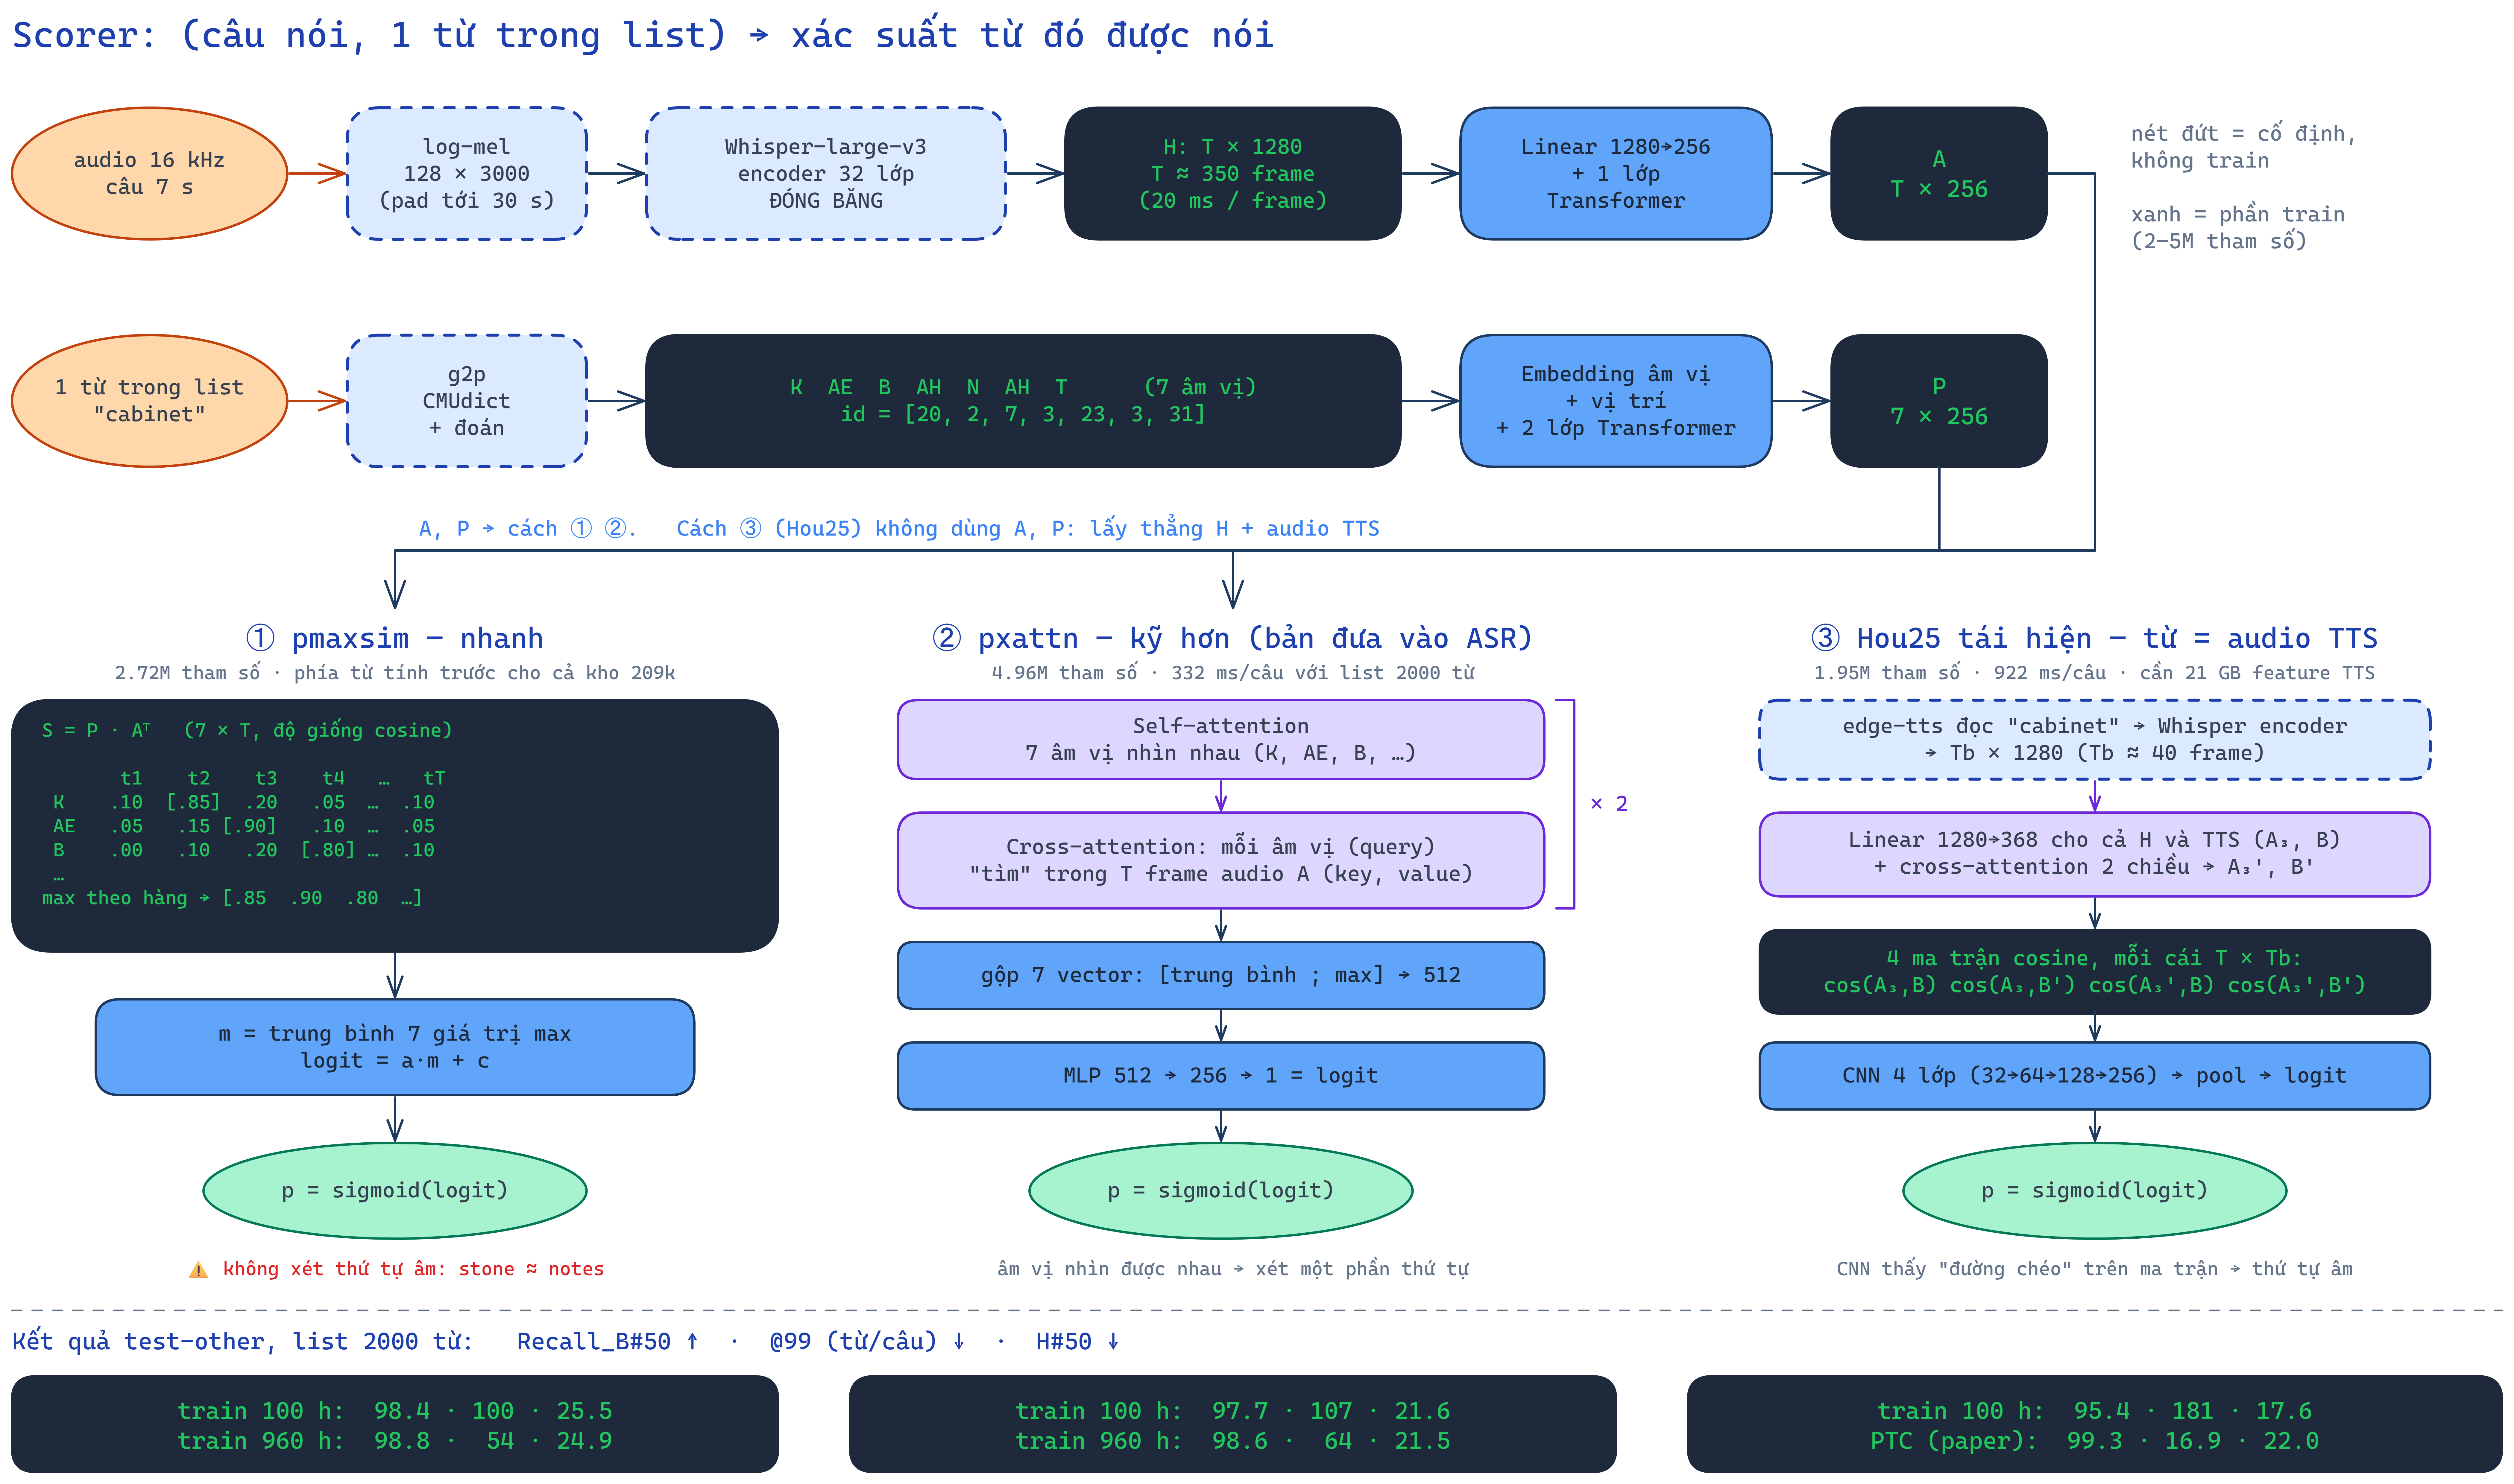
\includegraphics[width=\linewidth,height=0.86\textheight,keepaspectratio]{../2026-10-23/imgs/scorer_detail.png}
\end{frame}

\begin{frame}{Lựa chọn (a): âm vị thay audio TTS}
\begin{columns}[T]
\begin{column}{0.48\textwidth}
\nbox{\textbf{Hou25 phải trả giá gì cho TTS:}\\
-- đọc TTS cả kho 209k từ: khoảng 80 phút, \textbf{21 GB} feature;\\
-- từ mới (ngoài kho) phải TTS thêm: 2.7\% từ test không có TTS \src{Hoàng F8};\\
-- 1 giọng TTS (nữ) cho mọi người nói.}
\vspace{0.12cm}
\nbox{\textbf{Âm vị:} g2p ra ngay cho từ bất kỳ, không có ``giọng''. Phía từ của biến thể pmaxsim tính trước được cho cả kho.}
\end{column}
\begin{column}{0.48\textwidth}
\centering\scriptsize\setlength{\tabcolsep}{3pt}
\begin{tabular}{lcc}
\toprule
test-other N2000 & Hou25 \src{Hoàng} & pxattn\\
\midrule
từ đúng lọt top-50 (\#50) $\uparrow$ & 97.43 & \good{97.71}\\
số từ cần giữ 99\% (@99) $\downarrow$ & 256.4 & \good{106.7}\\
từ nghe giống lọt top-50 $\downarrow$ & \good{17.26} & \bad{21.58}\\
thời gian / câu & 922 ms & \good{332 ms}\\
giọng nữ / nam & \multicolumn{2}{c}{không chênh (CI chứa 0)}\\
\bottomrule
\end{tabular}\par
\vspace{0.15cm}\raggedright
\nbox[block body alerted]{\textbf{Đánh đổi:} tìm từ đúng ngang hoặc hơn, rẻ hơn nhiều; nhưng \bad{dễ bị từ nghe giống lừa hơn}. Giả thuyết (chưa kiểm): CNN trên ma trận frame $\times$ frame của Hou25 thấy được thứ tự âm chi tiết hơn.}
\end{column}
\end{columns}
\end{frame}

\begin{frame}{Sao không dùng ASR âm vị để hai phía cùng là âm vị (như PTC)?}
\centering\scriptsize\setlength{\tabcolsep}{4pt}
\begin{tabular}{L{2.6cm}L{5.4cm}L{5.4cm}}
\toprule
 & \textbf{(a) Âm vị $\leftrightarrow$ âm vị} \src{PTC-Bias §2.3--2.4} & \textbf{(b) Âm vị $\leftrightarrow$ vector audio} \src{pxattn}\\
\midrule
Audio thành gì & \textbf{xác suất 71 âm vị} mỗi frame: chỉ giữ ``âm gì'' & \textbf{vector 256 chiều} mỗi frame: giữ nguyên những gì Whisper nghe được\\
Train cái gì, bằng nhãn gì & bộ nhận dạng âm vị, nhãn \textbf{âm vị} (từ g2p của transcript) & bộ so khớp, nhãn \textbf{``từ có được nói không''}: đúng việc cần làm\\
Ra điểm thế nào & khớp CTC đúng chuỗi g2p + \textbf{luật chỉnh tay} ($\beta$, $\tau$, $\eta$, $K$, $M$) & \textbf{học thẳng}, chỉ 1 ngưỡng $p$\\
Khi phát âm thật lệch g2p & đường khớp phải theo đúng chuỗi g2p \ra{} bị trừ điểm & attention \textbf{học được} cách chịu lệch\\
\bottomrule
\end{tabular}\par
\vspace{0.2cm}\raggedright
\begin{columns}[T]
\begin{column}{0.49\textwidth}
\nbox{\textbf{Số ủng hộ (b):}\\
-- (a) phụ thuộc chất lượng bộ âm vị: PTC đổi WavLM sang encoder Qwen thì B-WER \bad{4.10 / 7.76 \ra{} 4.45 / 8.61} \src{PTC Bảng 1}.\\
-- g2p không phải ``chuẩn'': \textbf{11--16\%} từ hiếm có phát âm g2p khác MFA \src{ta đo, REPORT Q2}.}
\end{column}
\begin{column}{0.49\textwidth}
\nbox[block body alerted]{\textbf{Số ủng hộ (a):} PTC tìm từ tốt hơn: \#50 99.3, @99 16.9, so với pxattn 960 h 98.6 / 63.9. Nhưng khác encoder (WavLM), khác data \ra{} \hi{chưa so công bằng}.\\
\textbf{S0:} làm (a) trên \textbf{cùng encoder Whisper, cùng data}. Tiêu chí viết trước.}
\end{column}
\end{columns}
\end{frame}

\begin{frame}{Lựa chọn (b): mỗi âm vị dùng attention tự tìm mình trong audio}
\begin{columns}[T]
\begin{column}{0.52\textwidth}
\centering
\begin{tikzpicture}[font=\scriptsize,>={Stealth}]
\foreach \k in {0,...,13} {\draw[fill=SoftBlue,draw=Primary!50] (0.42*\k,0) rectangle ++(0.38,0.5);}
\node[anchor=west] at (0,0.8) {350 ô audio (mỗi ô 20 ms), ví dụ vẽ 14 ô};
\fill[Accent] (0.42*4,0) rectangle ++(0.38,0.5);
\fill[Accent!60] (0.42*5,0) rectangle ++(0.38,0.5);
\node[draw=Primary,fill=white,rounded corners=2pt] (k) at (1.2,-1.4) {âm vị \textbf{K}};
\node[draw=Primary,fill=white,rounded corners=2pt] (t) at (4.5,-1.4) {âm vị \textbf{T}};
\draw[->,thick,Accent!80!black] (k) -- (0.42*4+0.19,-0.05) node[midway,left]{70};
\draw[->,Accent!80!black] (k) -- (0.42*5+0.19,-0.05) node[midway,right]{20};
\fill[Accent] (0.42*11,0) rectangle ++(0.38,0.5);
\draw[->,thick,Accent!80!black] (t) -- (0.42*11+0.19,-0.05) node[midway,right]{75};
\node[anchor=west,align=left] at (0,-2.3) {Mỗi âm vị có \textbf{100 điểm chú ý} rải lên các ô.\\Ô nào nghe giống mình thì dồn nhiều điểm.};
\end{tikzpicture}\par
\vspace{0.15cm}\raggedright
\nbox{\textbf{Hình attention vẽ đúng bảng ``rải điểm'' này:} hàng = âm vị của từ, cột = ô audio, màu sáng = nhiều điểm. Các trang sau đọc hình này.}
\end{column}
\begin{column}{0.45\textwidth}
\nbox{\textbf{Làm gì với điểm đã rải:} mỗi âm vị mang về thông tin của các ô mình dồn điểm. 7 âm vị đều tìm được chỗ khớp, theo đúng thứ tự \ra{} $p$ cao.}
\vspace{0.08cm}
\nbox{\textbf{Vì sao không dùng CNN như Hou25:} Hou25 so audio với audio nên vệt chéo \textbf{có sẵn} cho CNN nhìn. Âm vị $\times$ ô audio ban đầu \textbf{không có vệt nào}, nên phải để từng âm vị tự đi tìm.}
\vspace{0.08cm}
\nbox[block body alerted]{\textbf{Điểm then chốt:} model chỉ được dạy ``từ có được nói không'', \textbf{không ai dạy vị trí}. Nhưng muốn đoán đúng thì phải rải điểm đúng chỗ \ra{} \hi{bảng rải điểm tự trở thành bản đồ vị trí}.}
\end{column}
\end{columns}
\end{frame}

\begin{frame}{Cách đọc hình attention lớp 1: từ ``bastard'' (test-clean)}
\centering
\begin{tikzpicture}
\node[anchor=south west,inner sep=0] (img) at (0,0) {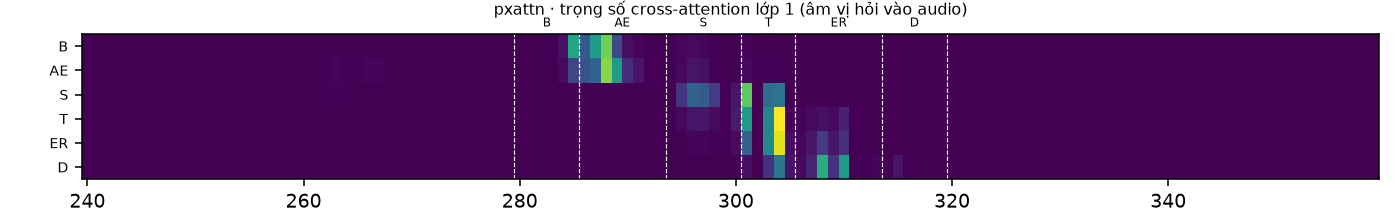
\includegraphics[width=0.98\linewidth]{imgs/bastard_l1.png}};
\begin{scope}[x={(img.south east)},y={(img.north west)},font=\scriptsize,>={Stealth}]
\draw[->,RiskRed,thick] (-0.01,1.12) node[above,align=center,text=RiskRed]{hàng = 6 âm vị của từ (g2p)} -- (0.035,0.7);
\draw[->,RiskRed,thick] (0.47,1.18) node[above,text=RiskRed]{chữ trên + vạch trắng = âm vị thật trong audio (MFA)} -- (0.47,0.92);
\draw[->,RiskRed,thick] (0.62,-0.22) node[below,text=RiskRed]{cột = ô audio, mỗi ô 20 ms (frame 280 $\approx$ giây 5.6)} -- (0.62,0.08);
\end{scope}
\end{tikzpicture}\par
\vspace{0.45cm}\raggedright
\begin{columns}[T]
\begin{column}{0.32\textwidth}
\nbox{\textbf{1. Cả câu tối}, chỉ sáng ở frame 283--311 ($\approx$ 5.7--6.2 s): đúng chỗ ``bastard''.}
\end{column}
\begin{column}{0.32\textwidth}
\nbox{\textbf{2. Bậc thang:} B, AE \ra{} S \ra{} T \ra{} ER, D: \textbf{đúng thứ tự}.}
\end{column}
\begin{column}{0.32\textwidth}
\nbox[block body alerted]{\textbf{3. Chưa hoàn hảo:} B sáng ở đầu AE; ER sáng cùng chỗ T (lệch sang đoạn kề).}
\end{column}
\end{columns}
\end{frame}

\begin{frame}{Đối chứng 2: cosine thô trong cùng model = nhiễu}
\centering\scriptsize
\textbf{``bastard''} cosine thô\par
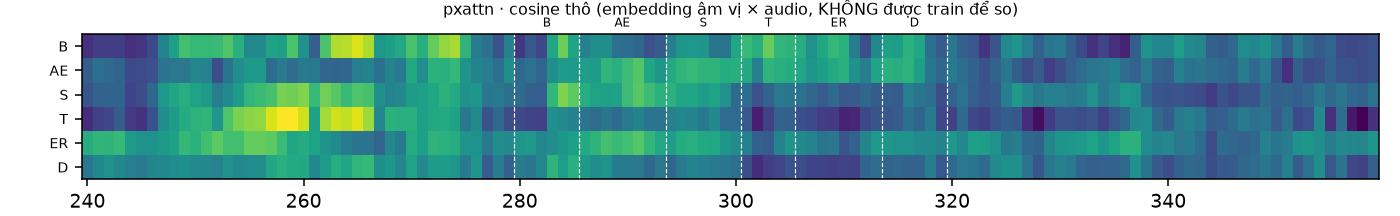
\includegraphics[width=0.84\linewidth]{imgs/bastard_cos.png}\par
\textbf{``uncommon''} cosine thô\par
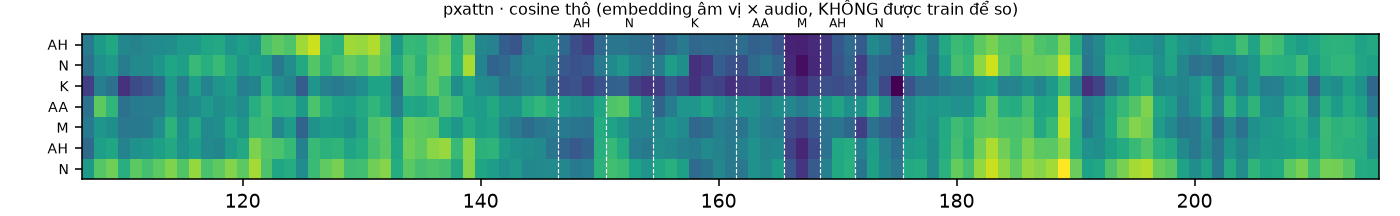
\includegraphics[width=0.84\linewidth]{imgs/uncommon_cos.png}\par
\vspace{0.15cm}\raggedright
\begin{columns}[T]
\begin{column}{0.48\textwidth}
\nbox{\textbf{Là gì:} lấy thẳng vector âm vị và vector audio \textbf{của chính pxattn}, tính độ giống (cosine), không qua attention.}
\end{column}
\begin{column}{0.48\textwidth}
\nbox[block body alerted]{\textbf{Thấy gì:} sáng lung tung, cả ngoài từ. Trúng span 8.8 / 12.3\%, \textbf{ngang ngẫu nhiên} (10.2 / 12.4\%). \ra{} Bậc thang chỉ có ở phép so đã học.}
\end{column}
\end{columns}
\end{frame}

\begin{frame}{Tổng hợp bằng số: vị trí là thứ scorer học ra thật}
\centering\small\setlength{\tabcolsep}{5pt}
\begin{tabular}{L{6.4cm}ccc}
\toprule
Phép thử (so với mốc MFA; clean / other) & \textbf{lớp 1} & cosine thô & ngẫu nhiên\\
\midrule
Đỉnh của từ rơi trong span của từ & \good{99.5 / 99.2\%} & 8.8 / 12.3\% & 10.2 / 12.4\%\\
Phần điểm chú ý nằm trong từ & \good{0.87 / 0.84} & -- & 0.07 / 0.08\\
Sai số vị trí từ (trung vị) & \good{0.03 / 0.03 s} & 2.54 / 2.05 s & 2.52 / 1.95 s\\
Âm vị có đỉnh đúng đoạn của nó ($\sim$0.1 s) & \good{66.9 / 64.5\%} & 1.3 / 1.8\% & 1.2 / 1.4\%\\
Hạng ô chéo, ma trận 39$\times$39 & \good{1.5} & 21.2 & $\approx$ 20\\
Từ đúng có $p<0.5$ vẫn trúng span & \good{100 / 94\%} & & \\
\bottomrule
\end{tabular}\par
\vspace{0.3cm}\raggedright
\begin{columns}[T]
\begin{column}{0.48\textwidth}
\nbox{\textbf{Vì sao tin được:} nhãn train chỉ là ``có/không''; mốc MFA chưa từng thấy; cùng model mà cosine thô ngang ngẫu nhiên.}
\end{column}
\begin{column}{0.48\textwidth}
\nbox[block body alerted]{\textbf{Giới hạn:} 400 câu/tập ($\sim$1.000 từ), 1 checkpoint, MFA tự sai 10--20 ms.}
\end{column}
\end{columns}
\end{frame}

\begin{frame}{Lựa chọn (c): sigmoid \ra{} xác suất dùng được làm ngưỡng}
\begin{columns}[T]
\begin{column}{0.54\textwidth}
\centering\scriptsize\setlength{\tabcolsep}{3pt}
\textbf{Qwen3-ASR-1.7B, list N2000, B-WER} \src{wnorm}\par\vspace{0.05cm}
\begin{tabular}{lc}
\toprule
không context & 7.40 / 16.08\\
nguyên list N2000 & 7.40 / 16.45\\
pxattn top-50 (cách của Hou25) & 5.71 / 11.57\\
\textbf{pxattn lọc $p\geq0.5$} & \good{4.78 / 9.71}\\
oracle (chỉ từ đúng) & 4.01 / 7.73\\
\midrule
list toàn nhiễu (\texttt{missing\_N2000}) \ra{} $p\geq0.5$ & 7.39 / 16.18\\
\bottomrule
\end{tabular}\par
\vspace{0.15cm}
\begin{tabular}{lcc}
\toprule
cần bao nhiêu từ để giữ 99\% từ đúng & Hou25 & pxattn\\
\midrule
test-other N2000 (@99) $\downarrow$ & 256.4 & \good{106.7}\\
\bottomrule
\end{tabular}
\end{column}
\begin{column}{0.43\textwidth}
\nbox{\textbf{Vì sao:} top-50 luôn đưa 50 từ, kể cả khi câu không có từ hiếm nào. Xác suất độc lập cho phép \textbf{số từ thay đổi theo câu}, kể cả \textbf{0 từ}.}
\vspace{0.1cm}
\nbox{\textbf{Bằng chứng:} lọc ngưỡng tốt hơn top-50 rõ, gần oracle. List toàn nhiễu thì scorer đưa Qwen về đúng mức không context (7.39 so với 7.40): \good{không bị list nhiễu kéo sai}.}
\vspace{0.1cm}
\nbox[block body alerted]{\textbf{Giới hạn:} Whisper với prompt 0--1 từ bị \bad{lặp chữ}, nên trên Whisper vẫn phải dùng top-50 (phụ lục B).}
\end{column}
\end{columns}
\end{frame}

% ==================================================================
\section{Kết quả}
\begin{frame}{Scorer: kết quả chính}
\begin{columns}[T]
\begin{column}{0.53\textwidth}
\centering\scriptsize\setlength{\tabcolsep}{3pt}
\textbf{Whisper-turbo, top-50, B-WER} \src{chuẩn hoá plain}\par\vspace{0.05cm}
\begin{tabular}{lcc}
\toprule
 & N100 & N2000\\
\midrule
nguyên list & 8.04 / 13.98 & 9.15 / 18.69\\
Hou25 \src{số paper} & 5.4 / 10.0 & 5.8 / 11.7\\
Hou25 tái hiện \src{Hoàng} & \good{4.4 / 8.7} & \good{4.9 / 9.2}\\
\textbf{pxattn} \src{pipeline Hoàng} & 4.6 / 9.0 & 5.1 / 10.1\\
\bottomrule
\end{tabular}\par\vspace{0.2cm}
\textbf{Qwen3-ASR-1.7B, N2000} \src{wnorm}\par\vspace{0.05cm}
\begin{tabular}{lcc}
\toprule
 & WER & B-WER\\
\midrule
nguyên list & 1.69 / 3.55 & 7.40 / 16.45\\
\textbf{pxattn lọc $p\geq0.5$} & \good{1.32 / 2.68} & \good{4.78 / 9.71}\\
oracle (chỉ từ đúng) & 1.22 / 2.43 & 4.01 / 7.73\\
\texttt{missing\_N2000} \ra{} $p\geq0.5$ & 1.65 / 3.42 & 7.39 / 16.18\\
\bottomrule
\end{tabular}
\end{column}
\begin{column}{0.44\textwidth}
\nbox{\textbf{Khác Hou25 đúng 1 chỗ:} từ được biểu diễn bằng \hi{âm vị} thay vì audio TTS.}
\vspace{0.08cm}
\nbox{\textbf{So với nguyên list:} giảm có ý nghĩa thống kê, N2000 \good{$-$3.85 / $-$8.69}.}
\vspace{0.08cm}
\nbox{\textbf{List toàn nhiễu:} Qwen giữ đúng mức không context (7.39 so với 7.40).}
\vspace{0.08cm}
\nbox[block body alerted]{\textbf{Nói thẳng:} cùng pipeline, pxattn \bad{kém Hou25 tái hiện 0.2--0.9} (1 seed, chưa CI).}
\end{column}
\end{columns}
\end{frame}

\begin{frame}{Scorer: chốt đóng góp ở mức nào}
\begin{columns}[T]
\begin{column}{0.50\textwidth}
\centering\scriptsize\setlength{\tabcolsep}{3pt}
\begin{tabular}{lccc}
\toprule
test-other N2000 & R\_B\#50 $\uparrow$ & R\_B@99 $\downarrow$ & R\_H\#50 $\downarrow$\\
\midrule
Hou25 (Hoàng) & 97.43 & 256.4 & \good{17.26}\\
pxattn 100 h & 97.71 & 106.7 & \bad{21.58}\\
pxattn 960 h & \good{98.59} & \good{63.9} & \bad{21.47}\\
PTC-Bias \src{paper} & 99.30 & 16.9 & 22.00\\
\bottomrule
\end{tabular}\par\vspace{0.05cm}\raggedright
{\scriptsize\color{TextGray} \#50: từ đúng lọt top-50. @99: cần bao nhiêu từ để giữ 99\% từ đúng. H\#50: từ nghe giống lọt top-50.}\par
\vspace{0.2cm}\footnotesize
\begin{tabular}{L{2.6cm}cc}
\toprule
 & Hou25 & pxattn\\
\midrule
cần TTS & có & \good{không}\\
thời gian/câu & 922 ms & \good{332 ms}\\
lọc theo ngưỡng & khó (@99 256) & \good{được} (@99 107)\\
vị trí & 0.06 s & \good{0.03 s, tới âm vị}\\
\bottomrule
\end{tabular}
\end{column}
\begin{column}{0.46\textwidth}
\nbox[block body alerted]{\textbf{Claim chốt:} chính xác \textbf{gần bằng} Hou25, recall bằng hoặc hơn; đổi lại \hi{không cần TTS, nhanh hơn khoảng 3 lần, có $p$ để lọc, có vị trí}. Không claim ``thắng Hou25''.}
\vspace{0.15cm}
\nbox{\textbf{Cái scorer có mà Hou25 không có:} $p$ hiệu chỉnh (lọc theo ngưỡng được) và vị trí tới mức âm vị, đúng hai thứ cần cho bước can thiệp lúc decode.}
\vspace{0.15cm}
\nbox{\textbf{Còn mở:} so ghép cặp với Hou25 (chờ file Hoàng); âm vị--âm vị thật (S0) chưa chạy, xem trang sau.}
\end{column}
\end{columns}
\end{frame}

% ==================================================================
\section{Còn lại}
\begin{frame}{Để chốt scorer: còn thiếu gì}
\centering\scriptsize\setlength{\tabcolsep}{4pt}
\begin{tabular}{cL{5.0cm}L{4.0cm}L{2.0cm}L{1.6cm}}
\toprule
\# & Việc & Trả lời câu nào & Chi phí & Trạng thái\\
\midrule
\textbf{S0} & \textbf{Âm vị--âm vị} (cách của PTC): head CTC âm vị trên cùng encoder Whisper, cùng data; chấm bằng khớp CTC. Thêm pxattn 1 lớp & sao không dùng ASR âm vị? lớp 2 có cần không? & GPU $\sim$10 h \src{ước lượng} & \bad{chưa}\\
S1 & So ghép cặp với Hou25 (Hoàng), có khoảng tin cậy & khoảng 0.2--0.9 có thật không, do đâu & CPU, nửa ngày & \bad{chờ file Hoàng}\\
S2 & Bỏ ứng viên chồng thời gian (giữ từ $p$ cao hơn). \src{PTC §2.4 đã có cơ chế tương tự} & dùng vị trí sửa được lỗi từ nghe giống không & GPU $\sim$2 h & chưa\\
S3 & Decode lại Whisper với list sau S2 & khoảng cách với Hou25 có đóng lại không & GPU $\sim$3 h & chưa\\
S4 & 3 seed kiến trúc được chọn & phương sai do train & GPU 3 $\times$ 5 h & chưa\\
\bottomrule
\end{tabular}\par
\vspace{0.25cm}\raggedright
\begin{columns}[T]
\begin{column}{0.48\textwidth}
\nbox{\textbf{Tiêu chí S0, viết trước khi chạy:} đổi sang âm vị--âm vị nếu \#50 $\geq$ pxattn, từ nghe giống không tệ hơn, sai số vị trí $\leq$ 0.05 s. Không đạt thì giữ pxattn.}
\end{column}
\begin{column}{0.48\textwidth}
\nbox{\textbf{Bước sau} (theo gợi ý của thầy buổi 1/11): dùng $p$ và vị trí của scorer khi can thiệp lúc decode. Scorer nào thắng S0 cũng cho được cả $p$ và vị trí.}
\end{column}
\end{columns}
\end{frame}

\begin{frame}{Xin thầy góp ý}
\begin{enumerate}\setlength{\itemsep}{8pt}
\item Cách trình bày đóng góp của scorer: \textbf{``gần bằng Hou25, không cần TTS, nhanh gấp 3, có $p$ để lọc, có vị trí''} đã đủ thuyết phục chưa?
\item Lý do chọn âm vị + attention (3 lựa chọn + các cách đã bỏ) còn thiếu bằng chứng nào thầy muốn thấy?
\item \textbf{S0} (âm vị--âm vị bằng ASR âm vị): chạy trước khi chốt, giới hạn khoảng 1 tuần?
\item Xin card GPU cố định cho S0--S4 (khoảng 30 h \src{ước lượng}).
\end{enumerate}
\end{frame}

% ==================================================================
\appendix
\section{Phụ lục}
\begin{frame}{Từng bộ phận: khác Hou25 ở đâu, vì sao, bằng chứng}
\centering\scriptsize\setlength{\tabcolsep}{3pt}
\begin{tabular}{L{1.5cm}L{2.2cm}L{2.4cm}L{4.0cm}L{4.2cm}}
\toprule
 & Hou25 \src{paper §2.2} & pxattn (nhóm) & Vì sao & Bằng chứng đã đo\\
\midrule
Biểu diễn từ & audio TTS qua encoder Whisper & \hi{âm vị g2p} + 2 lớp Transformer & không cần TTS; từ mới chấm ngay; phía từ không có ``giọng'' & 332 so với 922 ms/câu; giới tính: CI chứa 0 \\
\addlinespace
Phía audio & Whisper đóng băng + Linear & như Hou25 + 1 lớp Transformer & giữ encoder để \textbf{chỉ đổi 1 biến} & \bad{chưa ablation} lớp thêm \\
\addlinespace
So khớp & 4 ma trận cosine \ra{} CNN & \hi{âm vị là query}, cross-attention vào frame audio & âm vị không có thời lượng nên không có ``vệt chéo'' cho CNN bắt; để attention tự căn & lớp 1 tự căn âm vị \ra{} frame: sai số 0.03 s \\
\addlinespace
Gộp & average pool & [mean; max] theo âm vị & max giữ được một khớp ngắn trong câu dài & Hoàng F14: average pool làm loãng vệt ngắn \src{trên Hou25}\\
\addlinespace
Đầu ra & ``softmax ra điểm'' & \hi{sigmoid, BCE} từng cặp & xác suất độc lập: lọc theo ngưỡng, list được phép rỗng & Qwen: $p\geq0.5$ tốt hơn top-50 (4.78 / 9.71 so với 5.71 / 11.57)\\
\bottomrule
\end{tabular}\par
\vspace{0.25cm}\raggedright
\nbox{4.96M tham số, train trên train-clean-100 \textbf{đúng dữ liệu Hou25}, nên chênh lệch đến từ thiết kế, không từ dữ liệu. 3 trang sau đi vào 3 lựa chọn chính.}
\end{frame}

\begin{frame}{Thêm 3 từ khác: lớp 1 đều ra bậc thang}
\centering\scriptsize
\textbf{``refer''} (test-other) \hfill R \ra{} AH \ra{} F \ra{} ER\par
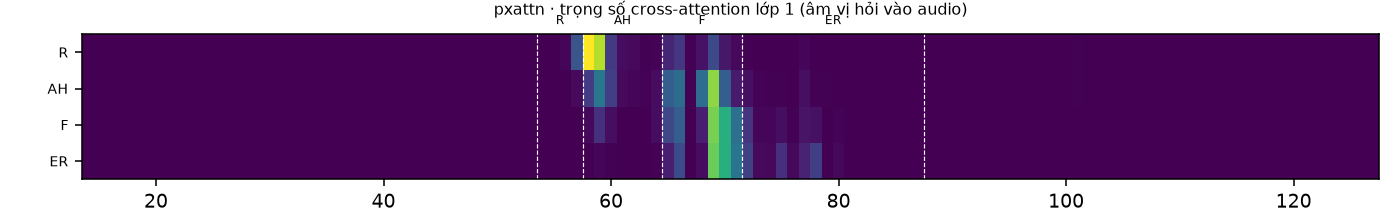
\includegraphics[width=0.72\linewidth]{imgs/refer_l1.png}\par
\textbf{``uncommon''} (test-other) \hfill AH, N \ra{} K, AA \ra{} M, AH, N\par
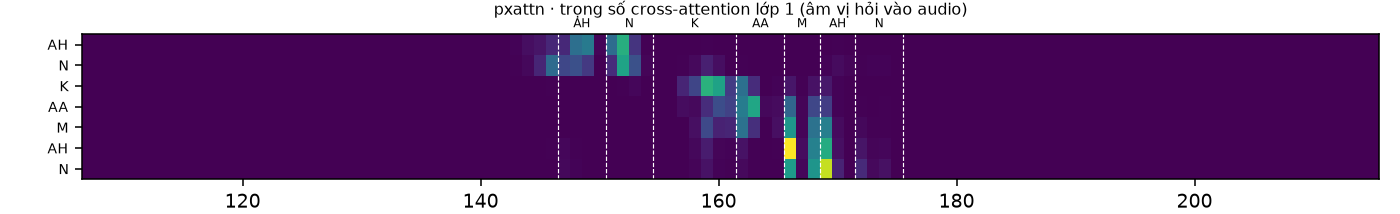
\includegraphics[width=0.72\linewidth]{imgs/uncommon_l1.png}\par
\textbf{``milner's''} (test-clean) \hfill M, IH \ra{} L \ra{} N \ra{} ER, Z\par
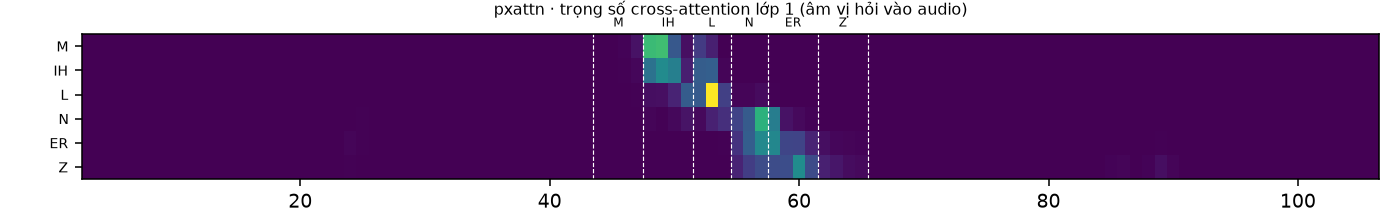
\includegraphics[width=0.72\linewidth]{imgs/milners_l1.png}\par
\raggedright
{\scriptsize\color{TextGray} Ví dụ do script tự lấy từ mẫu ngẫu nhiên, không chọn tay.}
\end{frame}

\begin{frame}{Đối chứng 1: attention lớp 2 \textbf{không} còn là bản đồ vị trí}
\centering\scriptsize
\textbf{``bastard''} lớp 2\par
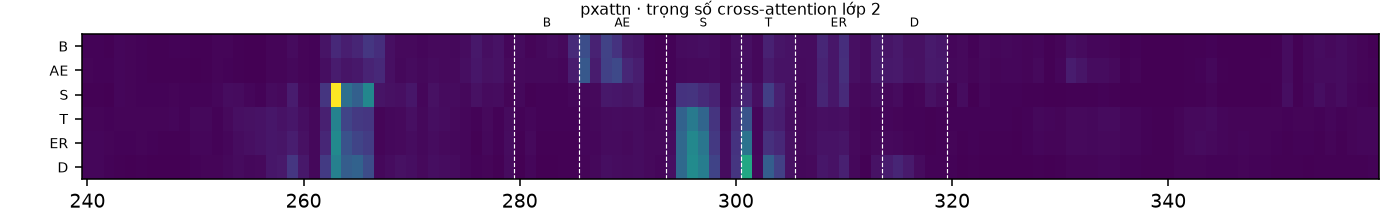
\includegraphics[width=0.84\linewidth]{imgs/bastard_l2.png}\par
\textbf{``uncommon''} lớp 2\par
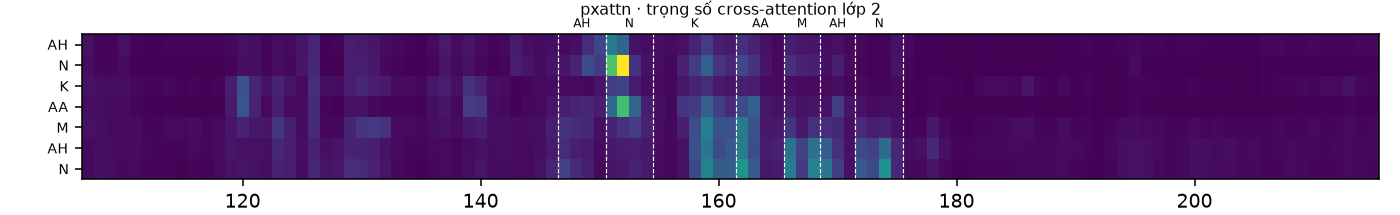
\includegraphics[width=0.84\linewidth]{imgs/uncommon_l2.png}\par
\vspace{0.15cm}\raggedright
\begin{columns}[T]
\begin{column}{0.48\textwidth}
\nbox{\textbf{Thấy gì:} điểm chú ý rải rộng, có chỗ sáng \textbf{ngoài từ} (``bastard'': hàng S sáng ở frame $\approx$263, trước từ). Không còn bậc thang.}
\end{column}
\begin{column}{0.48\textwidth}
\nbox{\textbf{Số đo:} chỉ $\sim$50\% từ có đỉnh trúng span (lớp 1: 99\%). \ra{} \hi{Vị trí chỉ đọc ở lớp 1.} \src{ta diễn giải: lớp 2 nhìn rộng ra ngữ cảnh}}
\end{column}
\end{columns}
\end{frame}

\begin{frame}{Ma trận 39$\times$39: âm vị nào nhìn vào âm vị nào (lớp 1)}
\begin{columns}[T]
\begin{column}{0.44\textwidth}
\centering
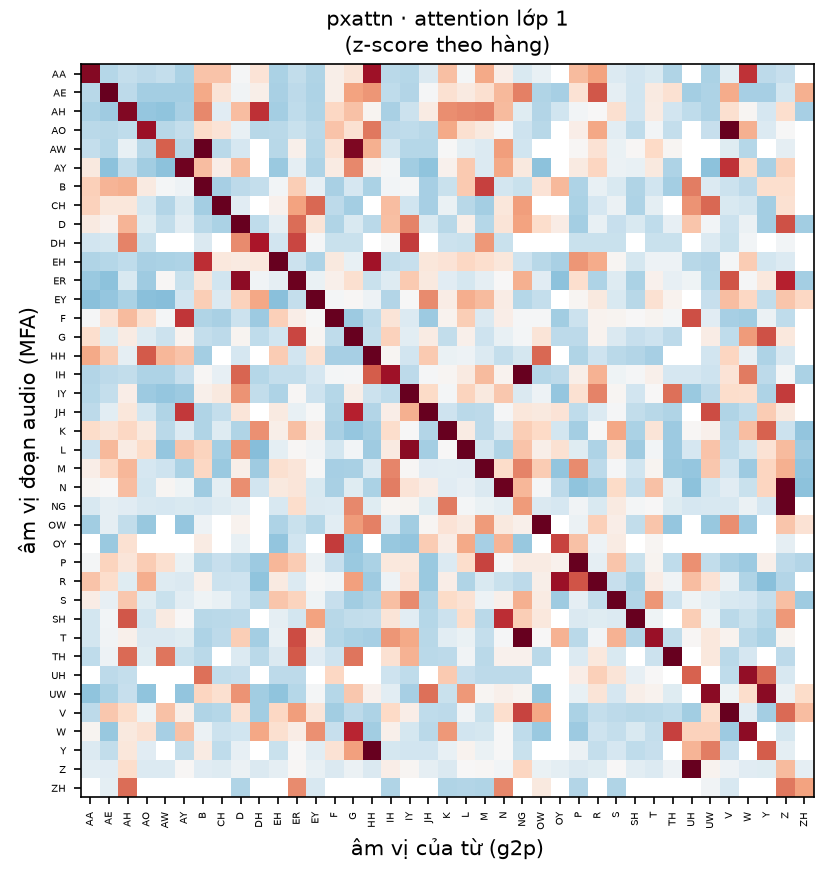
\includegraphics[width=\linewidth,height=0.84\textheight,keepaspectratio]{imgs/phone_matrix_l1.png}
\end{column}
\begin{column}{0.54\textwidth}
\nbox{\textbf{Cách tạo:} đoạn audio là âm X (MFA): âm Y của từ dồn bao nhiêu điểm vào đó? Cộng trên mọi từ, chuẩn hoá theo hàng.}
\vspace{0.08cm}
\nbox{\textbf{Cách đọc:} hàng = âm \textbf{thật trong audio}; cột = âm \textbf{đang đi tìm}; đỏ = nhìn vào nhiều.}
\vspace{0.08cm}
\nbox[block body alerted]{\textbf{Thấy gì:} \hi{đường chéo đỏ}: AE đi tìm thì dồn vào đoạn AE, K vào K\ldots{} 69\% hàng có ô chéo lớn nhất (hạng TB 1.5 / 39). Lớp 2: 5\%; cosine thô: 0\%.}
\vspace{0.08cm}
{\scriptsize\color{TextGray} Giới hạn: trong một từ, ``cùng loại âm'' thường cũng là ``cùng chỗ'', nên hai thứ này lẫn vào nhau.}
\end{column}
\end{columns}
\end{frame}

\begin{frame}{Đã thử và bỏ}
\centering\scriptsize\setlength{\tabcolsep}{3pt}
\begin{tabular}{L{3.6cm}L{4.6cm}L{5.6cm}}
\toprule
Đã thử & Số chính & Vì sao bỏ / giữ\\
\midrule
\textbf{hxattn}: cho scorer nhìn thêm hyp lần 1 của Qwen & Qwen B-WER \bad{6.58 / 14.07} (pxattn 4.78 / 9.71) & Nghi học tắt theo hyp thay vì nghe audio \ra{} \textbf{bỏ}.\\
\addlinespace
\textbf{Loss theo cả list} (1 từ đúng + 200 nhiễu) thay BCE & \#50 94.95, @99 \bad{518.8} (pxattn 97.71 / 106.7) & Tệ mọi metric, nghi tín hiệu từ đúng bị pha loãng \ra{} \textbf{bỏ}.\\
\addlinespace
\textbf{Chốt cứng qua chữ ASR} (hypmatch: chữ Qwen \ra{} âm vị \ra{} so) & \#50 \bad{95.41}, từ nghe giống \bad{35.70} & Sai ở bước ASR là mất luôn \ra{} \textbf{bỏ}.\\
\addlinespace
\textbf{pmaxsim}: mỗi âm vị lấy frame giống nhất, không attention & \#50 98.44, từ nghe giống 25.52; B-WER không khác pxattn có ý nghĩa & Rẻ: phía từ tính trước cho cả kho \ra{} \textbf{giữ làm tầng lọc rẻ}. Không xét thứ tự âm (stone $\approx$ notes).\\
\addlinespace
Train 960 h thay 100 h & \#50 \good{98.59}, @99 \good{63.9} & Thêm dữ liệu giúp. Bảng chính vẫn dùng 100 h để so công bằng với Hou25.\\
\bottomrule
\end{tabular}\par
\vspace{0.1cm}\raggedright
{\scriptsize\color{TextGray} Số chọn từ: test-other N2000. Ngoài ra đã thử chuẩn hoá điểm theo câu: @99 tệ hơn \ra{} bỏ.}
\end{frame}

\begin{frame}{Scorer đã gần trần: lỗi còn lại nằm ở ASR}
\centering\scriptsize\setlength{\tabcolsep}{4pt}
\begin{tabular}{lcccc}
\toprule
Whisper, test-other & B-WER & \textbf{nghe giống} & từ đúng rớt khỏi prompt & từ nhiễu viết đè\\
\midrule
không prompt & 18.92 & 10.24 & -- & --\\
\textbf{oracle (chỉ từ đúng)} & -- & \textbf{4.62} & -- & --\\
pxattn N100 & 8.92 & \textbf{4.69} & 0.04 & 0.07\\
pxattn N2000 & 10.00 & \textbf{4.32} & 1.68 & 0.34\\
\bottomrule
\end{tabular}\par
\vspace{0.05cm}
{\scriptsize\color{TextGray} Phân rã B-WER theo nguồn gốc lỗi (\texttt{bench/error\_breakdown.py}). Nghe giống = từ viết ra cách từ đúng $\leq$ 2 âm vị. test-clean: pxattn N2000 nghe giống 2.50, oracle 2.33.}\par
\vspace{0.25cm}\raggedright
\begin{columns}[T]
\begin{column}{0.48\textwidth}
\nbox{\textbf{Ví dụ:} audio nói \textit{``Bartley''}, từ này \textbf{đã có trong prompt}, Whisper vẫn viết \textit{``Bartly''}: chính tả quen hơn thắng. \src{ví dụ minh hoạ}}
\end{column}
\begin{column}{0.48\textwidth}
\nbox[block body alerted]{\textbf{Insight:} lỗi nghe giống của pxattn \textbf{ngang oracle} (4.69 so với 4.62). Prompt hoàn hảo cũng không sửa được \ra{} \hi{phải can thiệp lúc decode}. Nhóm này là \textbf{gần nửa} B-WER còn lại.}
\end{column}
\end{columns}
\end{frame}

\begin{frame}{Phụ lục A -- Khoảng tin cậy ghép cặp (Whisper)}
\centering\small\setlength{\tabcolsep}{6pt}
\begin{tabular}{lcc}
\toprule
$\Delta$B-WER = A $-$ B \src{95\% CI, bootstrap theo câu, 1.000 lần} & clean & other\\
\midrule
pxattn N100 $-$ nguyên list N100 & \good{$-$3.47} [$-$6.16; $-$1.90] & \good{$-$5.07} [$-$5.78; $-$4.42]\\
pxattn N2000 $-$ nguyên list N2000 & \good{$-$3.85} [$-$4.46; $-$3.26] & \good{$-$8.69} [$-$9.63; $-$7.78]\\
\midrule
pxattn N100 $-$ pmaxsim N100 & $-$0.03 [$-$0.28; +0.21] & $-$1.38 [$-$5.57; +0.39]\\
pxattn N2000 $-$ pmaxsim N2000 & $-$0.17 [$-$0.53; +0.17] & $-$0.37 [$-$0.89; +0.14]\\
\midrule
pxattn $-$ Hou25 (Hoàng) & \bad{chưa có} & \bad{chưa có}\\
\bottomrule
\end{tabular}\par
\vspace{0.3cm}\raggedright
\nbox{pxattn và pmaxsim chưa phân biệt được về B-WER. Chọn pxattn vì có \textbf{vị trí tới mức âm vị}, không phải vì B-WER tốt hơn.}
\end{frame}

\begin{frame}{Phụ lục B -- Các thí nghiệm khác}
\centering\scriptsize\setlength{\tabcolsep}{3pt}
\begin{tabular}{L{3.3cm}L{5.6cm}L{5.3cm}}
\toprule
Câu hỏi & Số chính & Insight\\
\midrule
Prompt chỉ có từ đúng (Whisper, N100) & oracle: B-WER 5.12 nhưng WER \bad{20.08} (clean) & Prompt 0--1 từ làm Whisper \textbf{lặp chữ} (khoảng 30 câu). Cách model dùng list là nút thắt riêng. Qwen không bị.\\
\addlinespace
Nguyên list ở N lớn (Whisper) & N$\geq$1000: chỉ 2--6\% từ đúng còn trong prompt & Whisper chỉ giữ 223 token cuối: list không vừa prompt.\\
\addlinespace
Giới tính giọng \src{biên bản 24/10} & 44 nữ / 29 nam (ước từ F0); mọi CI chứa 0 & Không thấy ảnh hưởng; scorer âm vị không có ``giọng'' ở phía từ.\\
\addlinespace
Câu nhiều từ hiếm \src{biên bản 24/10} & pxattn N100, câu $>$1 từ: 4.37 / 8.47; oracle 4.33 / 8.63 & Hưởng lợi đều.\\
\addlinespace
hxattn (scorer nhìn thêm hyp lần 1) & 6.58 / 14.07 (Qwen) & Kém: nghi học tắt theo hyp \ra{} bỏ.\\
\bottomrule
\end{tabular}
\end{frame}

\end{document}
